% =====================================================================
%  Người C -- Task 5: Sprint 2, kiểm thử, CI/CD và bàn giao
%  Nguồn: docs/test-scenarios/test-scenarios.md, apps/api/test/, apps/web/tests/,
%         tests/e2e/, docker-compose.yml, docs/deployment.md, docs/figures/as2/
%  Ngân sách: ~7 trang
% =====================================================================
\section{Task 5 -- Sprint 2, CI/CD và bàn giao}

\subsection{Task 5.1 -- Hoàn thiện MVP end-to-end}

% TODO(C): 1 đoạn dẫn + bảng 7 nhóm chức năng (chi tiết/size-topping, giỏ, auth JWT,
% tạo đơn, thanh toán ZaloPay, trạng thái/lịch sử, validate 2 đầu).
\begin{table}[H]
\centering\small
\caption{Chức năng hoàn thiện trong Sprint 2}
\label{tabC:features}
\begin{tabularx}{\textwidth}{@{}l X l@{}}
\toprule
\textbf{Nhóm} & \textbf{Nội dung} & \textbf{Mã FR} \\
\midrule
% TODO(C)
\bottomrule
\end{tabularx}
\end{table}

\paragraph{Máy trạng thái đơn hàng.}
% TODO(C): sơ đồ + 1 đoạn: 7 trạng thái, chuyển sai 409, optimistic lock,
% huỷ đơn hoàn kho/điểm một lần, PAID cần refund thủ công.
% Nguồn: docs/order/state-machine.md

\subsection{Giao diện thực tế}

\begin{figure}[H]
\centering
\shot{../figures/as2/view/01-menu-mobile.png}{Thực đơn}
\hfill
\shot{../figures/as2/view/02-chi-tiet-size-topping.png}{Chọn size, topping}
\hfill
\shot{../figures/as2/view/03-gio-hang-mobile.png}{Giỏ hàng}
\caption{Luồng chọn món trên điện thoại}
\label{figC:ui-menu}
\end{figure}

\begin{figure}[H]
\centering
\shot{../figures/as2/view/04-dang-nhap-mobile.png}{Đăng nhập}
\hfill
\shot{../figures/as2/view/05-checkout-mobile.png}{Điểm và voucher}
\hfill
\shot{../figures/as2/view/06-thanh-toan-zalopay-mobile.png}{Chọn ZaloPay}
\caption{Đăng nhập, áp dụng điểm tích luỹ và chọn thanh toán}
\label{figC:ui-checkout}
\end{figure}

\begin{figure}[H]
\centering
\shot{../figures/as2/view/07-tao-giao-dich-zalopay.png}{Liên kết ZaloPay}
\hfill
\shot{../figures/as2/view/08-lich-su-don-mobile.png}{Lịch sử đơn}
\hfill
\shot{../figures/as2/view/09-xac-nhan-don-mobile.png}{Chi tiết đơn}
\caption{Giao dịch ZaloPay Sandbox, lịch sử và chi tiết đơn}
\label{figC:ui-zalopay}
\end{figure}

\begin{figure}[H]
\centering
\shot{../figures/as2/view/10-admin-dashboard-mobile.png}{Tổng quan}
\hfill
\shot{../figures/as2/view/11-admin-don-hang-mobile.png}{Đơn hàng}
\hfill
\shot{../figures/as2/view/12-admin-kho-nguyen-lieu-mobile.png}{Kho nguyên liệu}
\caption{Khu vực quản trị}
\label{figC:ui-admin}
\end{figure}

\begin{figure}[H]
\centering
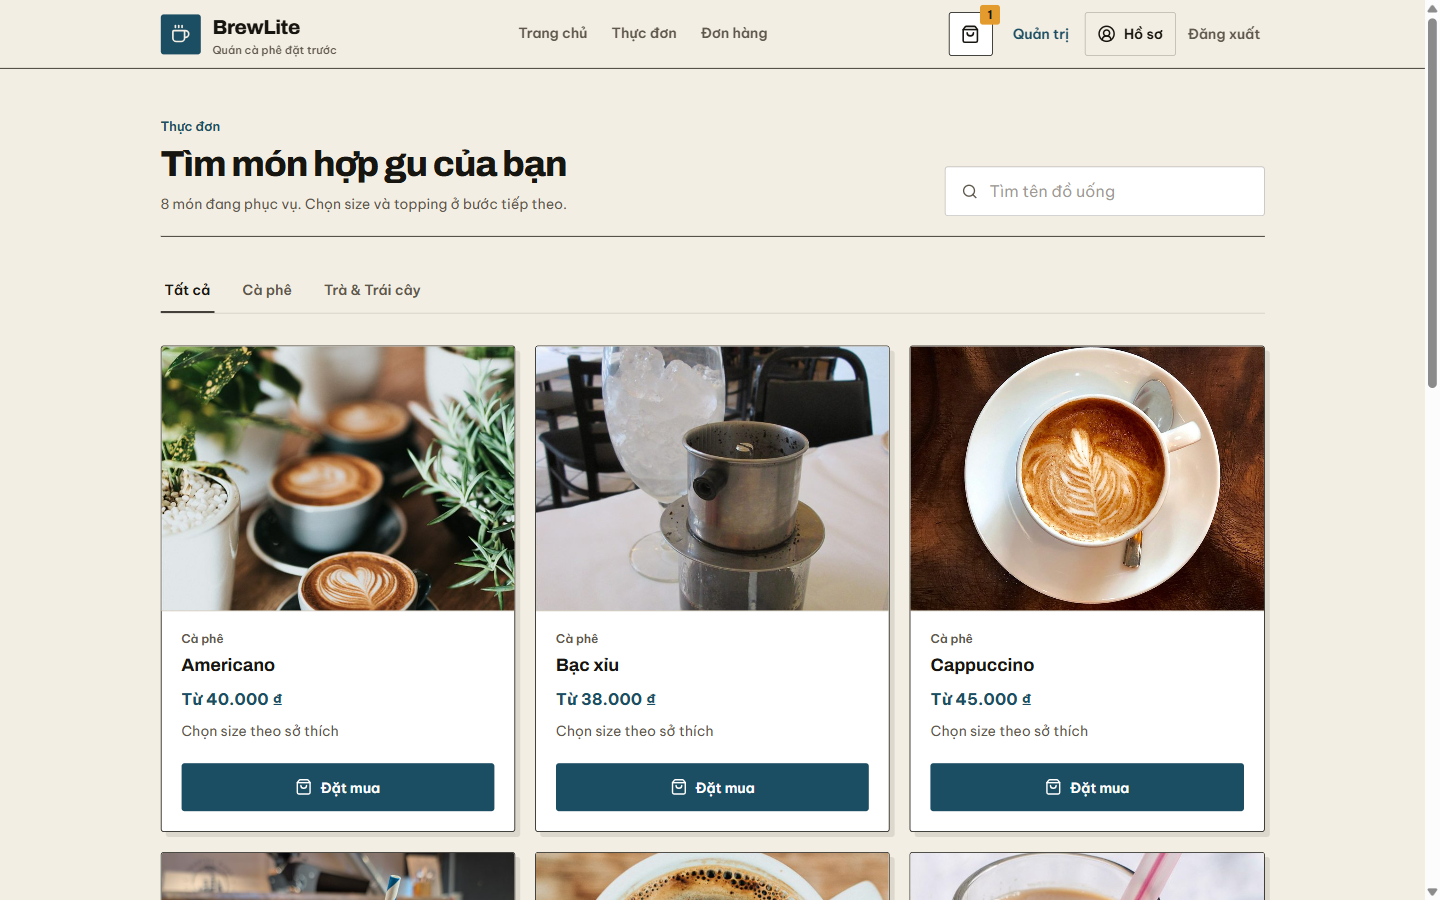
\includegraphics[width=0.94\textwidth]{../figures/as2/14-menu-desktop.png}
\caption{Thực đơn ở 1440$\times$900}
\label{figC:ui-desktop}
\end{figure}

\begin{figure}[H]
\centering
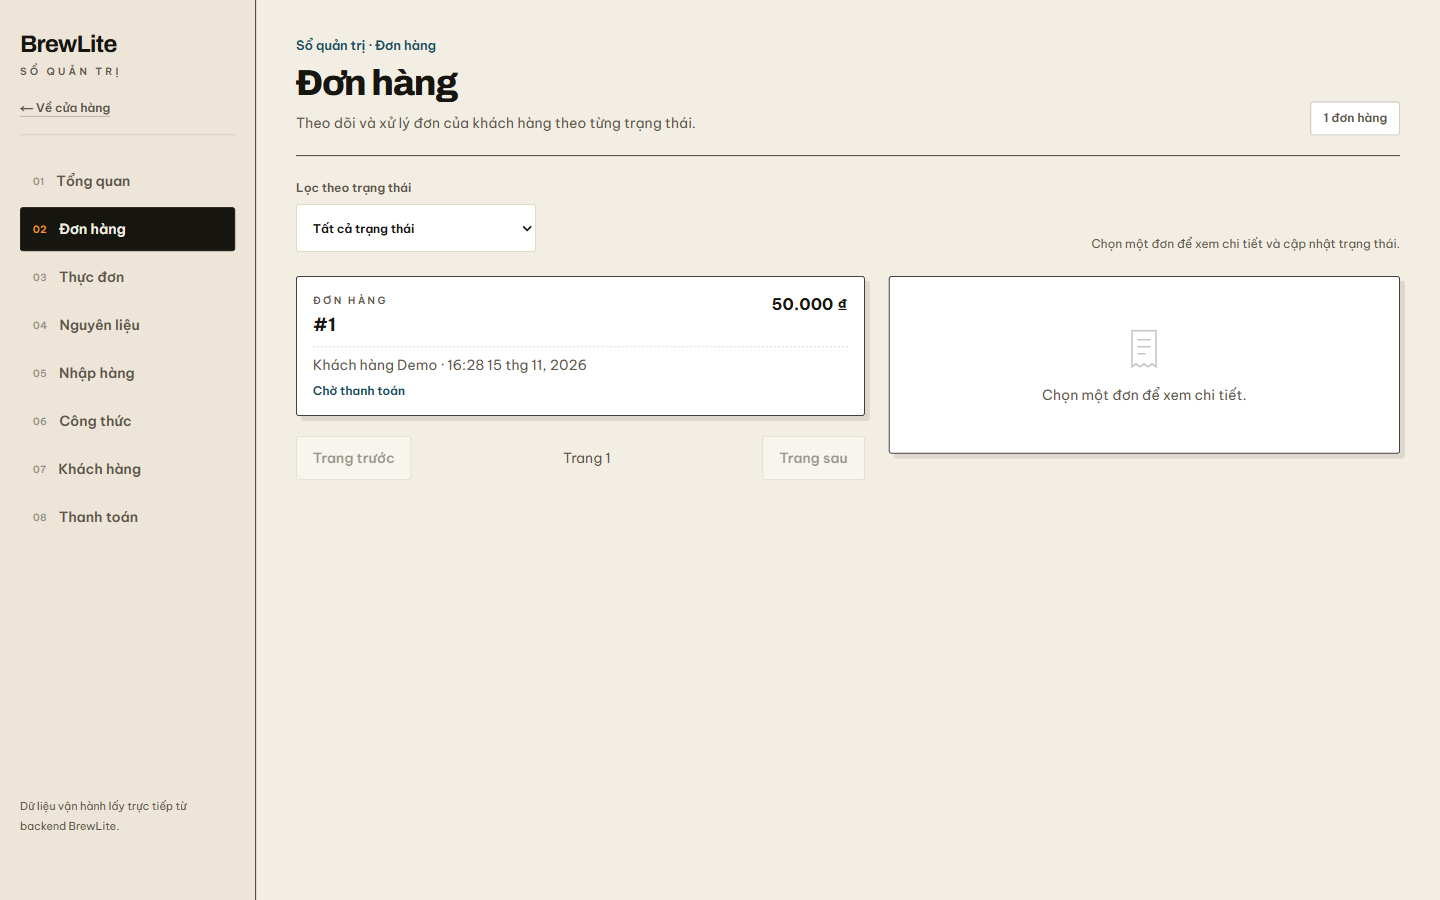
\includegraphics[width=0.94\textwidth]{../figures/as2/15-admin-don-hang-desktop.png}
\caption{Quản lý đơn hàng trên máy tính}
\label{figC:admin-desktop}
\end{figure}

\subsection{Task 5.2 -- Tích hợp và kiểm thử}

\paragraph{Kiểm thử tự động.}
% TODO(C): 1 đoạn: node:test, 15 tệp backend + 5 tệp frontend, schema PostgreSQL dùng một lần.
\begin{table}[H]
\centering\small
\caption{Nhóm kiểm thử và phạm vi}
\label{tabC:tests}
\begin{tabularx}{\textwidth}{@{}p{4.4cm} X c@{}}
\toprule
\textbf{Nhóm} & \textbf{Nội dung kiểm chứng} & \textbf{Số tệp} \\
\midrule
% TODO(C): 8 nhóm như as2.tex cũ
\bottomrule
\end{tabularx}
\end{table}

\begin{table}[H]
\centering\small
\caption{Kết quả chạy kiểm thử và build}
\label{tabC:results}
\begin{tabularx}{\textwidth}{@{}l X l@{}}
\toprule
\textbf{Hạng mục} & \textbf{Lệnh} & \textbf{Kết quả} \\
\midrule
% TODO(C): 49/49 backend, 10/10 frontend, build api/web, lint
\bottomrule
\end{tabularx}
\end{table}

\paragraph{Migration, seed và Docker Compose.}
% TODO(C): 1 đoạn + lệnh: docker compose up --build -d; prisma migrate deploy; prisma:seed.

\paragraph{Health check.}
% TODO(C): GET /api/v1/health trả JSON trạng thái API + DB; dùng cho smoke test và keep-alive.

\subsection{Task 5.3 -- Continuous Delivery/Deployment}
% TODO(C): QUAN TRỌNG -- repo hiện chỉ có .github/workflows/ci.yml + keepalive.yml,
% CHƯA có workflow CD. Viết trung thực:
%   - quality gate: lint + test + build (ci.yml);
%   - đóng gói: Dockerfile API; deploy: Render build từ Docker, Vercel Git integration;
%   - migration: prisma migrate deploy;
%   - smoke test: gọi /health sau deploy (thủ công/keep-alive);
%   - rollback: redeploy commit/tag trước trên Render/Vercel;
%   - phần chưa tự động: chưa có image tag GHCR, chưa có smoke test tự động, chưa rollback tự động.
% Nếu kịp: thêm cd.yml và chụp minh chứng; nếu không, ghi vào hạn chế.
\begin{table}[H]
\centering\small
\caption{Đối chiếu 7 yêu cầu pipeline CD của đề với hiện trạng}
\label{tabC:cd}
\begin{tabularx}{\textwidth}{@{}c X l@{}}
\toprule
\textbf{\#} & \textbf{Yêu cầu} & \textbf{Hiện trạng} \\
\midrule
% TODO(C): 7 dòng
\bottomrule
\end{tabularx}
\end{table}

\subsection{Task 5.4 -- Triển khai production và bàn giao}
% TODO(C): bảng URL frontend/API/health + tài khoản demo + release/tag + release notes.
% Sprint Review + Retrospective: 3 mục Đã tốt / Chưa tốt / Hành động.
% Video demo 3-5 phút: nêu link + các bước quay.
\begin{table}[H]
\centering\small
\caption{Địa chỉ bàn giao}
\label{tabC:urls}
\begin{tabularx}{\textwidth}{@{}l X@{}}
\toprule
\textbf{Hạng mục} & \textbf{URL / ghi chú} \\
\midrule
% TODO(C)
\bottomrule
\end{tabularx}
\end{table}

\begin{table}[H]
\centering\small
\caption{Sprint Retrospective}
\label{tabC:retro}
\begin{tabularx}{\textwidth}{@{}l X@{}}
\toprule
\textbf{Điểm} & \textbf{Nội dung} \\
\midrule
% TODO(C): điền 3 dòng retro
Đã làm tốt & \\
Chưa tốt & \\
Hành động & \\
\bottomrule
\end{tabularx}
\end{table}
